\chapter{Méthodes de représentation et d'analyse de l'architecture CxSOM}
\graphicspath{{03-Representation/}}
\minitoc

\section{Introduction}
Dans le chapitre précédent, nous avons proposé l'algorithme CxSOM, permettant de construire des architectures non-hiérarchiques de cartes auto-organisatrices. 

Dans ces architectures non-hiérarchiques, plusieurs cartes sont connectées et effectuent chacune une tâche d'apprentissage sur leur espace d'entrée externe, tout en prenant comme entrée secondaire les positions des \emph{Best Matching Unit} d'autres cartes. La particularité du modèle CxSOM est d'introduire des rétroactions entre cartes: l'architecture n'est pas un empilement de cartes qui apprennent tour à tour, de façon \emph{feedforward}.
Le but de ce modèle est de pouvoir construire des architectures assemblant un grand nombre de cartes; nous nous concentrons dans cette thèse sur des petites architectures de deux et trois cartes afin de comprendre les comportements qui émergent d'un tel système.

Nous étudions l'architecture CxSOM dans un cadre de mémoire associative.
L'objectif pour une architecture de cartes est alors d'apprendre une représentation des relations existant entre des entrées de différentes modalités, tout en apprenant une représentation de chaque espace d'entrée.
Le but de cette thèse est d'analyser comment est effectuée cette représentation des relations et des entrées dans une architecture CxSOM.
La compréhension du comportement de structures avec un faible nombres de cartes posera des bases pour la construction d'architectures plus grandes.

Ce système de cartes est un système complexe, même dans une architecture de quelques cartes. Chaque carte possède 500 unités; son état, représenté par son BMU, peut alors prendre 500 valeurs. L'état d'une carte dépend des cartes voisines.

Cette thèse s'inscrit dans une démarche complètement expérimentale: nous observons l'organisation d'architectures de cartes sur différents espaces d'entrées, différents configurations, différents paramètres pour comprendre leur comportement. Nous voulons également poser un formalisme clair sur des architectures de quelques cartes pour permettre l'adaptation de CxSOM à plus grande échelle.
Ce chapitre s'attelle à définir une méthode expérimentale claire et un formalisme pour cette méthode et pose les représentations utilisées.

Pour analyser l'organisation de ces cartes sur plusieurs entrées et plusieurs cartes, nous avons besoin de définir des représentations nouvelles par rapport à l'étude d'une SOM classique.
Nous posons dans ce chapitre la méthode expérimentale que nous utiliserons dans toutes les expériences présentées dans ce manuscrit. 
Nous présenterons des représentations adaptées à cette méthode expérimentale et le formalisme utilisé. Le but de ce chapitre est de présenter la démarche et expliciter les représentations choisies.
Nous introduirons enfin un indicateur caractérisant l'apprentissage de ces relations entre entrées, basé sur l'information mutuelle.
Toutes ces représentations seront illustrées sur une architecture de deux cartes.

\subsection{Une expérience simple à titre d'illustration}

La méthode expérimentale sera présentée dans toute ce chapitre sur l'exemple minimal d'une architecture de deux cartes. L'architecture est illustrée à droite en figure~\ref{fig:exp}: elle est composée de deux cartes en une dimension. Chaque carte prend une entrée externe. Il s'agit de $\inpx\m{1}=x$ et $\inpx\m{2}=y$, les coordonnées de points 2D sur un cercle. Ces deux modalités sont dépendantes: pour une valeur de $x$, seule deux valeurs sont possible pour $y$, et symétriquement. Les entrées sont représentées sur le schéma de gauche, figure~\ref{fig:exp}.
Ces entrées externes sont normalisées entre 0 et 1. Les deux cartes sont des lignes 1D de 500 n\oe{}uds. Les rayons de voisinage sont $h_e = 0.2$ et $h_c = 0.02$.
Chacune des deux cartes est également connectée à sa voisine, c'est-à-dire, la carte $M\m{1}$ prend en entrée contextuelle la position du BMU de $M\m{2}$, et inversement.
%es données relatives à cette expérience et le code permettant de faire les tracés sont fournies sur git.
Afin de comprendre les tracés que nous présenterons, nous utiliserons deux cartes de Kohonen classiques en tant que témoin.
Une carte prend en entrée les valeurs $x$, et la deuxième les valeurs $y$, mais ces cartes ne sont pas connectées entre elles. Les paramètres de ces cartes sont les mêmes que les cartes de CxSOM: 500 n\oe{}uds et $h_e = 0.2$.

\begin{figure}
\begin{minipage}{0.4\textwidth}
\centering
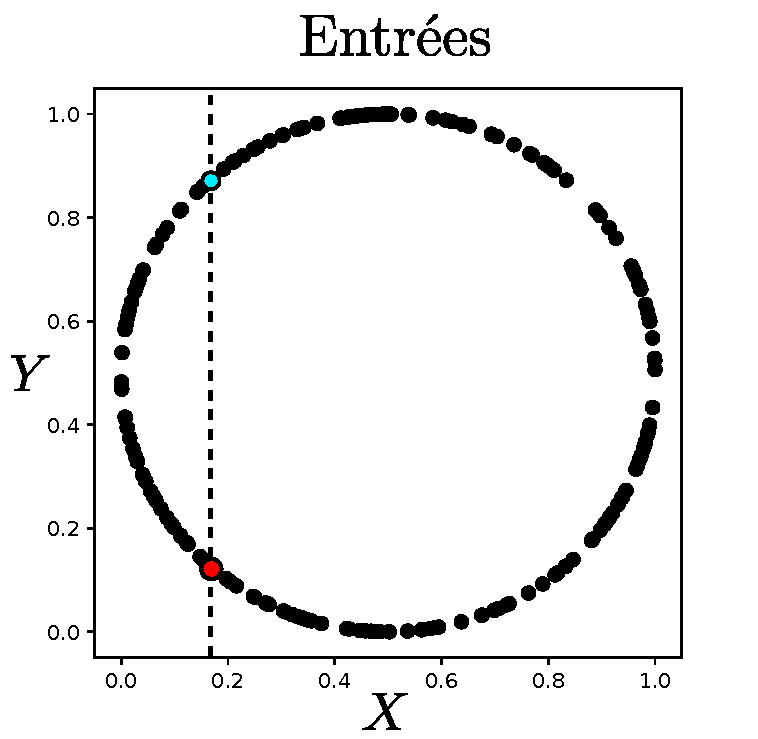
\includegraphics[width=0.8\textwidth]{2som_inp_noinformation}
\end{minipage}
\begin{minipage}{0.6\textwidth}
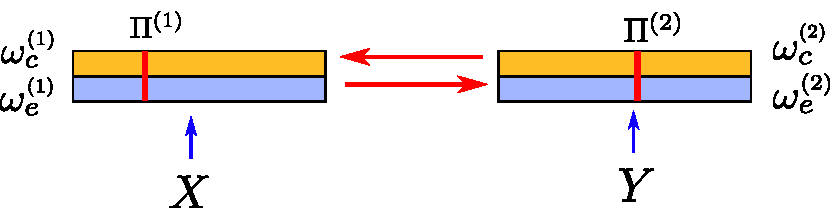
\includegraphics[width=\textwidth]{2som_archi}
\end{minipage}
\caption{Disposition des entrée, sous forme de cercle, à gauche, et architecture de deux cartes en une dimension étudiée et représentée dans ce chapitre.\label{fig:exp}}
\end{figure}

\subsection{Représentations et indicateurs classique des cartes de Kohonen}

Les cartes de Kohonen sont particulièrement associées à une facilité de représentation et de visualisation. Leur nombre réduit de prototypes et leur aspect topologique permet d'en tracer une représentation visuelle interprétable.
La manière la plus couramment utilisée de représenter une carte de Kohonen est de tracer les poids de ses prototypes, disposés dans le graphe (ligne ou grille) qu'est la carte. En fonction des dimensions des entrées, cette représentation prennent plusieurs formes. Deux exemples courants de représentation sont les suivants: 
\begin{itemize}
\item Le graphe qu'est la carte de Kohonen est représenté dans l'espace de ses positions (la grille d'indices $(i,j)$, ou une ligne indexée par $i$. Sur chaque noeud est tracé le poids correspondant. C'est le cas sur l'exemple de gauche en figure~\ref{fig:representation} dans lequel les poids des prototypes, qui sont des imagettes, sont affichés en chaque point de la grille. 
%Si la dimension d'un poids est trop grande pour être représentée graphiquement, il est également courant d'étiquetter chaque prototype et d'afficher ces étiquettes sur les n\oe{}uds de la carte, en tant que représentation.
\item Lorsque les données traitées sont des points deux ou trois dimensions, les poids des prototypes peuvent être directement tracés dans l'espace $\mathbb{R}^2$ ou $\mathbb{R}^3$. Ces poids sont alors reliés en fonction des positions des n\oe{}uds dans la carte, montrant ainsi la déformation de la carte dans l'espace d'entrée, c'est le cas sur l'exemple de droite en figure~\ref{fig:representation}.
\end{itemize}

Nous utiliserons des représentations adaptées au cas d'une architecture à plusieurs cartes à partir de ces deux modes de représentation. Cette adaptation dans le cas précis d'une architecture CxSOM est l'objet de cette section.

\begin{figure}
\begin{minipage}{0.5\textwidth}
\centering
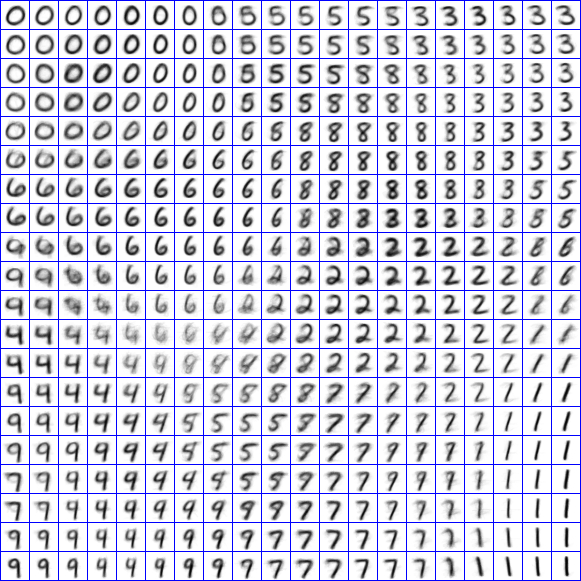
\includegraphics[width=0.5\textwidth]{digits.jpg}
\end{minipage}
\begin{minipage}{0.5\textwidth}
\centering
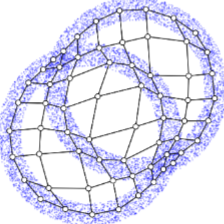
\includegraphics[width=0.5\textwidth]{points.png}
\end{minipage}
\caption{Représentations possible des poids d'une carte de Kohonen classiques, dans le cas d'entrées sous forme d'imagettes ou de points en deux dimensions.\label{fig:representation}}
\end{figure}

\subsection{Limites de la représentation classique pour CxSOM}

Utilisons d'abord les représentations classiques mentionnées ci-dessus pour tracer les poids de chacun des cartes d'une architecture CxSOM. Les poids sont tracés à la fin de l'apprentissage. La fin de l'apprentissage est définie comme le moment où les poids ont convergé vers une organisation restant stable au cours des itérations $t$.
La figure~\ref{fig:weights} présente le tracé des poids des deux cartes de l'exemple.
La courbe orange correspond aux poids externes, se dépliant sur chaque coordonnée $x$ et $y$ des points du cercle, appartenant chacune à $[0,1]$. Ce tracé permet d'observer que les poids externes couvrent l'intervalle $[0,1]$, et sont organisés de façon monotone, comme on l'attend dans une carte simple. Les poids contextuels, en bleu, ne présentent pas cette organisation monotone. Ils présentent toutefois une continuité: deux prototypes proches ont des poids proches. Le tracé nous informe donc sur le caractère continu de l'organisation de chacune de couches de poids. 

Notons que nous ne pouvons pas en tirer plus de conclusion: la représentation des poids de la figure~\ref{fig:weights} ne différencie pas les n\oe{}uds qui seront effectivement BMUs, des n\oe{}uds \emph{morts}. Ces n\oe{}uds morts ont bien un poids, mais ne seront jamais BMUs. Dans une carte de Kohonen classique, ces n\oe{}uds correspondent à des transitions, liant deux zones denses de l'espace d'entrée séparée par une zone sans points.
Par ailleurs, cette représentation concerne une seule carte. Nous ne pourrons pas tirer des informations sur l'influence des connexions entre cartes à partir de ces représentations.

Au regard des insuffisances des représentations classiques, que nous avons révélées sur un cas très simple de deux cartes mono-dimensionnelles, nous constatons qu'il est nécessaire de trouver un moyen de représenter l'architecture comme un tout. Nous devons définir une représentation qui montre comment l'architecture de cartes est capable d'apprendre les relations entre les entrées multimodales.

Même avec des représentations adaptées, l'analyse d'architecture comportant de nombreuses cartes ne peut pas simplement s'effectuer à l'aide de graphiques, qui deviendraient trop complexes.
La comparaison d'un grand nombre d'expériences est aussi difficilement réalisable graphiquement.
Cette difficulté de représentation et le besoin de comparer des expériences soulève la nécessité de définir une valeurs indicatrice du fonctionnement de la carte, que nous proposerons dans ce chapitre.

% Enfin, la représentation visuelle d'une cartes d'une architecture est limitée par la dimension des entrées et la dimension des cartes. Dans l'exemple, les entrées et les cartes sont en une dimension, représenter leurs poids est donc réalisable.
% En plus grande dimension, il sera nécessaire d'utiliser une représentation telle que celle décrite en figure~\ref{fig:representation}. Le nombre de connexions contextuelles limitera alors également la lecture d'un tracé. Cette difficulté de représentation soulève la nécessité de définir des valeurs indicatrices du fonctionnement de la carte, calculables en grande dimension.

\begin{figure}
\centering
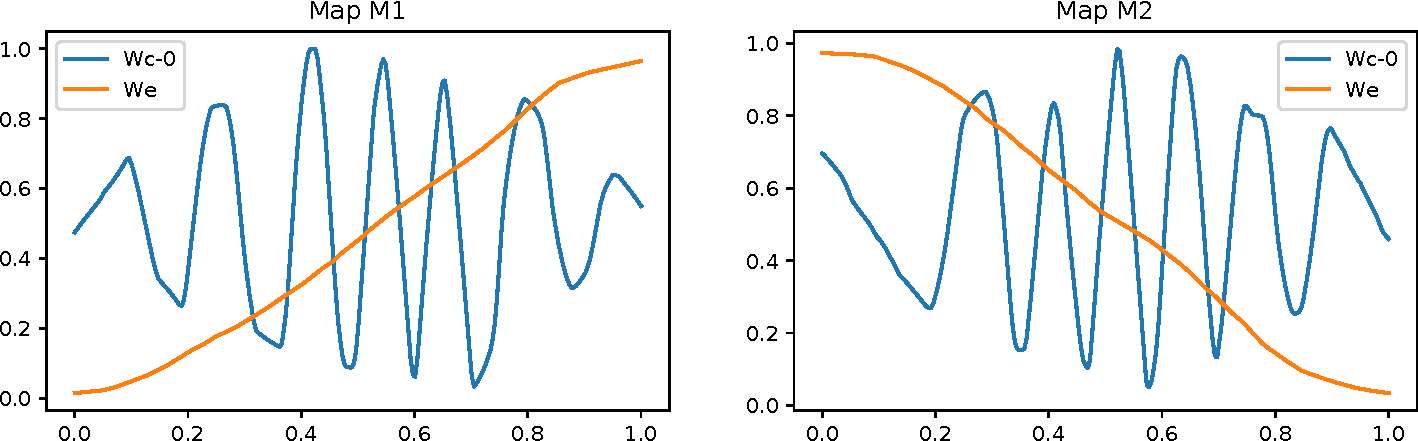
\includegraphics[width=0.9\textwidth]{weights_cercle1.pdf}

\caption{Représentation des valeurs des poids d'une carte au sein de CxSOM après apprentissage en fonction de leur position dans la carte. La seule représentation de ces poids ne suffit pas à savoir comment la carte se comporte.\label{fig:weights}}
\end{figure}

Ce chapitre questionne donc la façon de représenter une carte au sein d'une architecture. Nous présenterons en premier lieu le formalisme décrivant les cartes et leurs entrées multimodales associées ainsi que la méthode expérimentale que nous utiliserons pour toutes les expériences présentées dans cette thèse. A partir de ce formalisme, nous proposerons plusieurs représentations et indicateurs permettant de comprendre et représenter ce que calcule une architecture CxSOM sur les données d'entrées.

\section{Formalisation par variables aléatoires}

Nous introduisons dans cette section un formalisme traitant les éléments des cartes et les entrées en tant que variables aléatoires. 
Ce formalisme a à la fois l'avantage de clarifier les représentations et de permettre le développement d'indicateurs statistiques sur l'apprentissage effectué par les cartes.

\subsection{Représentation des entrées}
Sortons du problème illustratif à deux cartes pour revenir au cas général et formaliser davantage.
Nous nous plaçons dans une tâche de mémoire associative. 
Nous considérons plusieurs espaces d'entrée $\mathcal{D}\m{1},\cdots,\mathcal{D}\m{n}$ dont seront tirées les entrées présentées au cartes. Chaque espace est une modalité.
Les observations multimodales que l'on cherche à apprendre par l'architecture de cartes sont notées $(\inpx\m{i} \in \mathcal{D}\m{i}, i = 1 \cdots n)$. Ces observations $\inpx\m{i}$ sont modélisées comme des \emph{variables aléatoires}. Chaque variable aléatoire possède une distribution $p\m{i}$ sur $\mathcal{D}\m{i}$.
Nous notons $\mathbf{\inpx} = (\inpx\m{1}, \cdots, \inpx\m{n})$ la variable aléatoire jointe. Cette variable appartient à l'espace $\mathcal{D}\m{1} \times \cdots \times \mathcal{D}\m{n}$. Elle a une distribution jointe. La distribution de probabilité de chaque modalité $\inpx\m{i}$ sur son espace $\mathcal{D}\m{i}$ est alors une distribution marginale de $\mathbf{X}$.
A chaque pas de temps, un vecteur $\mathbf{\inpx} = (\inpx\m{0}_t, \cdots , \inpx\m{N}_t)$ est présenté à l'architecture: il s'agit d'une réalisation de la variable jointe $\mathbf{\inpx}$. On s'intéresse à l'apprentissage de relations entre entrées: les variables $\inpx\m{i}$ ne sont pas des variables indépendantes.

En pratique, ces variables sont des observations, issues par exemple de capteurs d'un robot. Ces observations sont issues d'un d'environnement général qui est modélisable. 
Nous introduisons la notion de \emph{modèle d'entrées} se rapportant à cette dépendance entre variables.
Le modèle d'entrée fait référence au modèle d'environnement permettant de générer les entrées multimodales fournies en entrées. Dans l'exemple d'illustration, les modalités sont les abscisses $\inpx\m{1} = x$ et les ordonnées $\inpx\m{2} = y$; le modèle d'entrées correspond à l'équation du cercle.

Le but de l'apprentissage non-supervisé par des cartes de Kohonen classiques est d'apprendre une représentation discrète de l'espace d'entrée.
Avec CxSOM, nous chercherons à la fois à apprendre un représentation discrète des espaces d'entrée mais aussi à apprendre une représentation du modèle d'entrées.

Les tracés et indicateurs que nous développerons dans cette section ont pour but de mesurer comment ce modèle d'entrées est appris par l'architecture. 

\subsection{Représentation du modèle d'entrée par une variable cachée}

Nous cherchons à évaluer expérimentalement la capacité du modèle CxSOM à apprendre à partir d'un environnement multimodal. Dans ce cadre expérimental particulier, nous choisissons des modèles d'entrées dont les relations sont connues. 
Nous utiliserons des modèles géométriques, comme le cercle présenté en section. Ces modèles peuvent être paramétrisés par une variable multidimensionnelle $U$. Les modalités sont définies comme des fonction de cette variable:
$\inpx\m{i} = f\m{i}(U)$
% L'exemple du cercle est ainsi paramétrisé par une variable U, représentant l'angle du point sur le cercle (à un facteur 2 pi près), selon l'équation paramétrique du cercle.
Cette représentation permet de dégager une nouvelle variable aléatoire représentant le modèle. Les entrées $X = (X1,..,Xn)$ sont en bijection avec $U$.
La définition de $U$ peut aussi être considérée comme un cas particulier de réduction de dimension du modèle. La variable multidimensionnelle $U$

Pour que la variable $U$ conserve toute l'information sur le modèle, la fonction $(f\m{1}, \cdots, f\m{N})$ : $(\inpx\m{1}, \cdots \inpx\m{N})\rightarrow U$ doit être une bijection. Toute valeur jointe d'entrée correspond à un seul $U$, toute valeur de $U$ renvoie à une seule valeur d'entrée jointe. 
Cet aspect est un cas particulier par rapport aux méthodes de réduction de dimension classique, car il n'y a pas de perte d'information.
Dans le cas d'exemple, $\mathbf{X} = (X,Y)$, les coordonnées cartésiennes des points du cercle est alors une vecteur aléatoire, dont les composantes sont les variables aléatoires $X,Y$. En définissant une variable $U$ à valeurs dans $[0,1]$, chaque point du du cercle peut maintenant s'écrire, selon l'équation paramétrique du cercle:
\begin{equation}
 \begin{cases}
     X = r  \cos(2\pi U)\\
     Y = r \sin(2 \pi U)
    \end{cases}\,.
\end{equation}

$U$ représente ici l'angle du point sur le cercle (à un facteur $2\Pi$ près). Les exemples donnés sont scalaires, mais cette représentation générale à n'importe quel dimension et nombre d'entrées.

Cette variable ajoute donc un attribut aux données échantillonnées durant une phase de test. Une phase de test donne donc un ensemble de valeurs de $U$, en plus des positions de BMUs $\bmu\m{i}$ et de leurs poids.


Ce modèle n'étant pas fourni à l'architecture de cartes lors de l'apprentissage, il s'agit d'un modèle \emph{latent}.
Nous cherchons, par l'architecture de cartes, a apprendre les entrées et les relations entre entrées: nous cherchons donc à extraire une structure dans le modèle latent. 

\begin{figure}
\centering
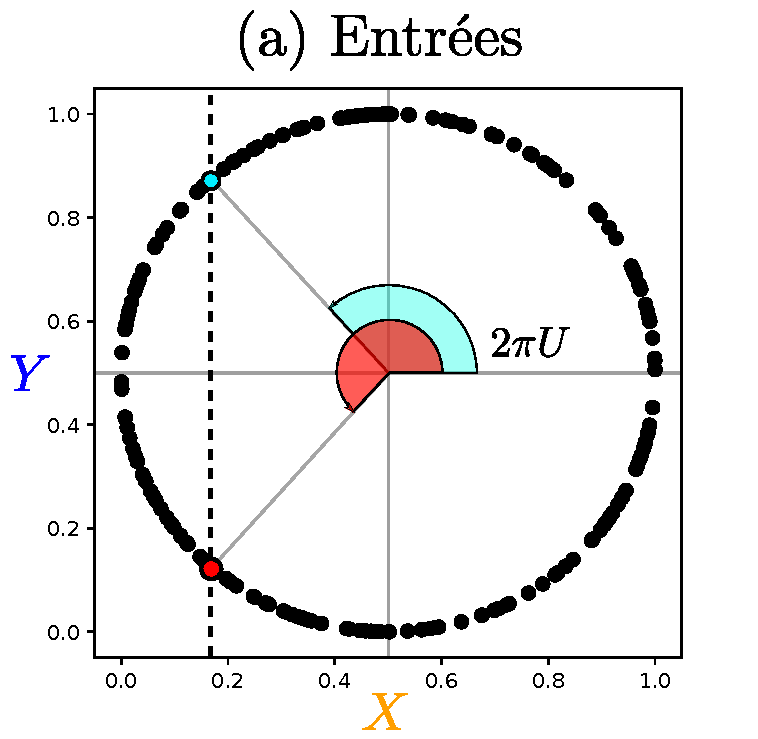
\includegraphics[width=0.6\textwidth]{2som_inp.pdf}
\caption{Représentation choisie pour le cercle. Le modèle auxquelles appartiennent les modalités $\inpx\m{1}$ et $\inpx\m{2}$ est représenté par la variable $U$. \label{fig:U}}
\end{figure}


\subsection{Démarche expérimentale}

Afin d'étudier le comportement de la carte à n'importe quel instant $t$ de l'apprentissage, nous effectuons une phase de \emph{test}, décrit en figure~\ref{fig:flowchart}
Lors de cette phase de test, des entrées sont présentées à la carte, mais seul le processus de recherche de la best matching unit est réalisé, les poids des cartes ne sont pas mis à jour. Cet étape génère un ensemble de réponses de la carte aux entrées présentées.
Les entrées utilisées lors du test sont un échantillon de taille 1000 de la variable aléatoire $(\inpx\m{1}, \cdots, \inpx\m{n})$.

Nous défissons a présent aussi des variables aléatoires pour chaque élément des cartes.
Nous représentons notamment les positions des BMUs par des variables aléatoires, $\bmu\m{1}, \cdots, \bmu\m{n}$ et leurs poids $\w\ext\m{1}(\bmu\m{1})$ et $\w\ext\m{2}(\bmu\m{2})$. 
Entre deux itérations de test, la valeur de ces éléments ne dépend que de l'entrée, car les poids ne sont pas mis à jour. Grâce à cette indépendance entre itération, les valeurs obtenues lors d'une phase de test forment un échantillon de la variable aléatoire jointe : 
$$(\inpx\m{1}, \cdots, \inpx\m{n}, \bmu\m{1}, \cdots, \bmu\m{n}, \w_e\m{1}(\bmu\m{1}), \cdots, \w_e\m{n}(\bmu\m{n}))$$

Les composantes de cette variable jointe ne sont pas indépendantes. Les représentations et indicateurs présentés ensuite chercheront à détecter et comprendre au mieux leurs dépendances statistiques.
Les variables d'entrées sont à valeurs continues et $\bmu$ à valeurs discrètes, correspondant aux 500 n\oe{}uds d'une carte. Nous considérerons cependant $\bmu$ comme une variable continue plutôt qu'une grandeur discrète. En effet, l'ensemble des positions du BMU correspondent une discrétisation de l'espace continu $[0,1]$, et sont ordonnées.
%Les échantillons de test utilisés dans cette partie contiennent 1000 éléments.
Le formalisme par variable aléatoires permet d'utiliser des outils et métriques issus de la théorie de l'information pour qualifier l'organisation des cartes au sein de l'architecture.

\begin{figure}
\centering
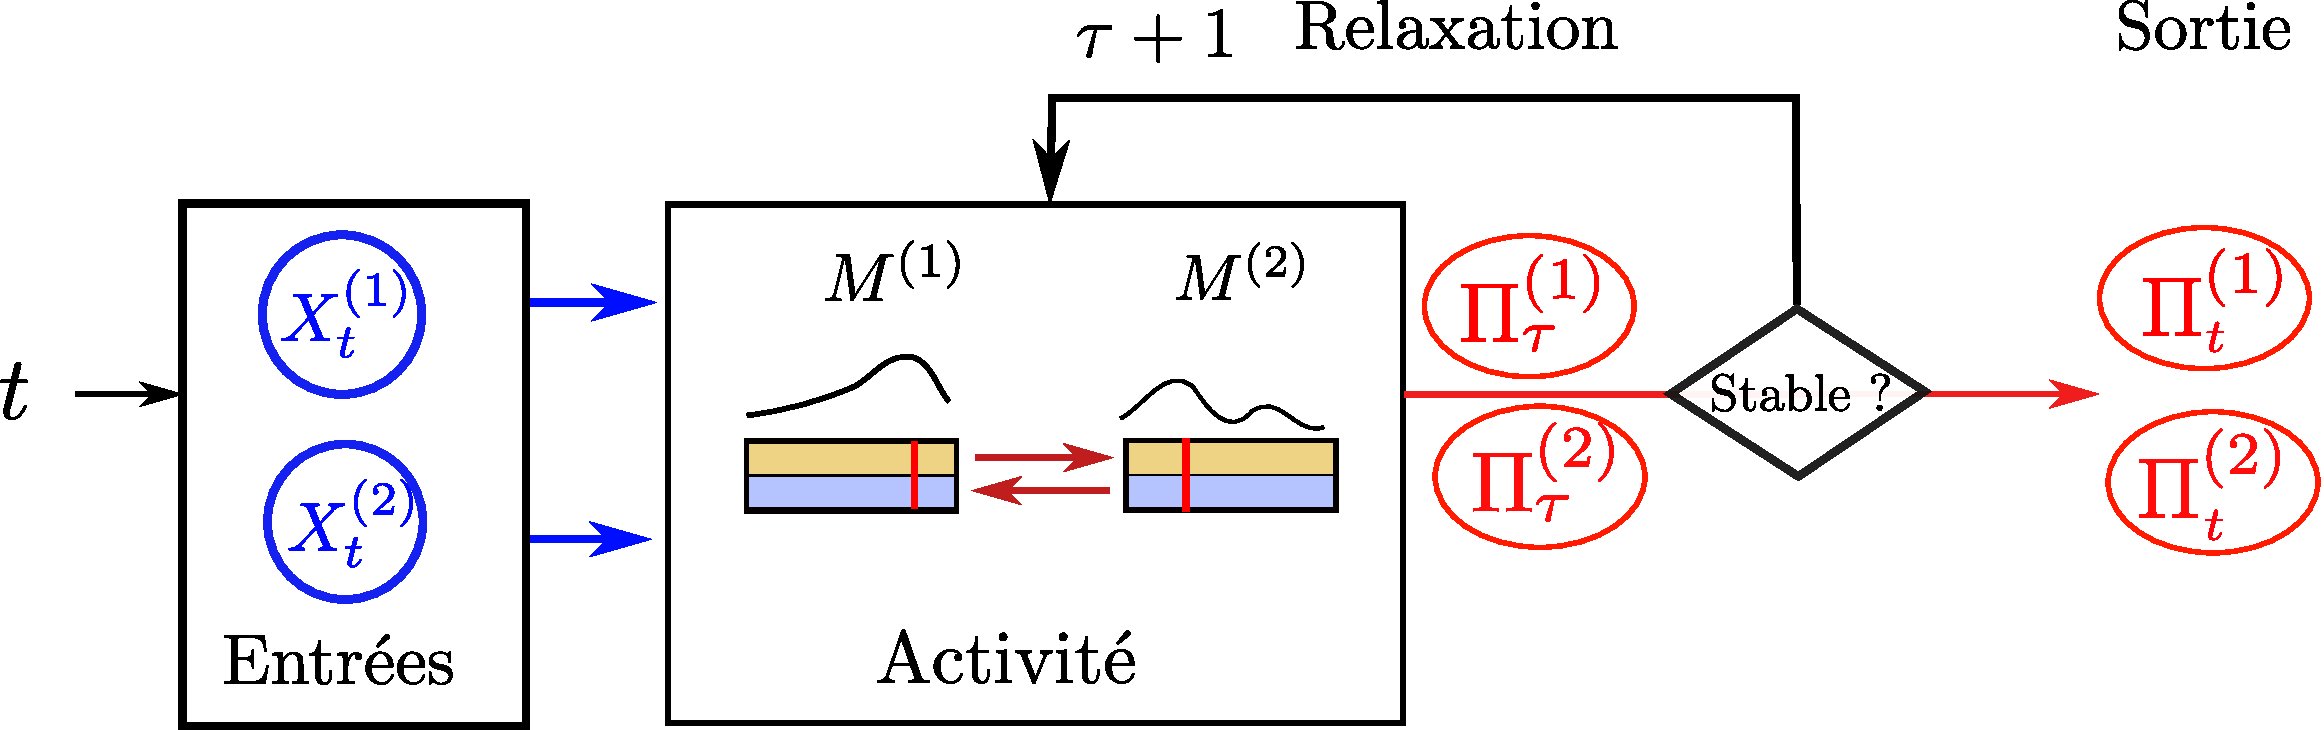
\includegraphics[width=0.85\textwidth]{tests_2maps.pdf}
\caption{Schéma decrivant les tests. Un test consiste à présenter successivement des réalisations de $mathbf{X}$, notées $(\inpx\m{1}_t,\inpx\m{2}_t)$. Nous laissons le processus de relaxation décrit au paragraphe xxx stabiliser les BMUs. Quand la stabilité est atteinte, la valeur des positions de BMU $\bmu\m{1}_t$ et $\bmu\ù{2}$ est obtenue. Un échantillon de test complet est obtenu en présentant un ensemble de réalisations de $\mathbf{X}$. Les poids ne sont pas mis à jour entre chaque itération, ce qui permet de considérer une phase de test comme un échantillonnage des variables aléatoires considérées: $\inpx\m{1},\inpx\m{2}$ par définition, mais aussi $\bmu\m{1}$, $\bmu\m{2}$ et $U$.}
\label{fig:flowchart}
\end{figure}

% \subsection{Résumé}
% Pour évaluer le comportement des cartes à une itération $t$, nous effectuons une phase de test sur les poids à cette itération. Cette phase de test consiste à enregistrer la réponse d'une carte à un grand nombre d'entrées test, sans effectuer de mise à jour des poids. Nous enregistrons ainsi les positions des BMUs résultats de chaque entrée présentées et leur poids externes.
% Les entrées et les réponses des cartes obtenues lors d'une phase de test sont modélisées comme des variables aléatoires, notées
% $$(\inpx\m{1}, \cdots, \inpx\m{n}, \bmu\m{1}, \cdots, \bmu\m{n}, \w_e\m{1}(\bmu\m{1}), \cdots, \w_e\m{n}(\bmu\m{n}))$$
% Une phase de test est un ensemble de réalisation de cette variables aléatoire jointe.

\section{Représentation graphiques}

A partir des échantillons de tests, nous proposons dans cette section les représentations graphiques que nous utiliserons et leur intérêt.
Il s'agit de tracer les dépendances entre les variables $$(\inpx\m{1}, \cdots, \inpx\m{N}, \bmu\m{1}, \cdots, \bmu\m{N}, \w_e\m{1}(\bmu\m{1}), \cdots, \w_e\m{N}(\bmu\m{N}))$$ dont un échantillon est obtenu lors du test.
Nous proposons d'abord une représentation pour évaluer la qualité de quantification vectorielle effectuée par une carte de l'architecture. Nous présenterons ensuite des représentations nous permettant de comprendre comment le modèle d'entrées est appris par l'architecture CxSOM.
% Ces points se superposent à la courbe de poids, mais certaines unités ne seront pas représentées: on les appelles \emph{unités mortes}. La position de la best matching unit $\bmu$ étant la réponse de la carte à une entrée, il s'agit d'un tracé d'un élément de la carte en fonction de la réponse de celle-ci.
%\subsection{Représentation des entrées par rapport au BMU}
\subsection{Erreur de quantification d'une modalité dans une carte}

La première fonction d'une carte de Kohonen est de réaliser une tâche de quantification vectorielle sur son entrée externe. Au sein d'une architecture de cartes, nous nous attendons à ce que chaque carte extrait une représentation de la modalité qu'elle prend en entrée.
Afin de mesurer cette qualité de la quantification vectorielle au sein d'une carte dans CxSOM, nous tracerons le nuage de points correspondant au poids externe du BMU $\w_e(\bmu\m{i})$ en fonction de l'entrée présentée $\inpx\m{i}$. Une carte effectue une quantification vectorielle correcte si ce nuage de points est proche de la fonction identité.
Ces tracés sont réalisés en figure~\ref{fig:erreur} pour l'expérience exemple. Ces tracés s'approchent de l'identité: la quantification des entrées est correctement réalisée.
On pourrait mesurer une erreur quadratique pour déterminer en quoi les points dérivent de l'identité, mais la représentation en nuage de points est, à défaut d'être quantitative, plus qualitative. En effet, ici, on observe que le nuage à une structure "filamenteuse". Nous reviendrons sur ce point par la suite, nous contentant de souligner ici que la représentation graphique exprime une propriété que la simple mesure d'erreur n'aurait pas mise en évidence. 

Cette représentation nous informe sur la qualité de quantification dans une seule carte relativement à une seule modalité. Il nous faut ensuite définir des méthodes de représentation permettant d'évaluer comment le modèle d'entrée est appris par l'architecture de cartes.

\begin{figure}
    \centering
    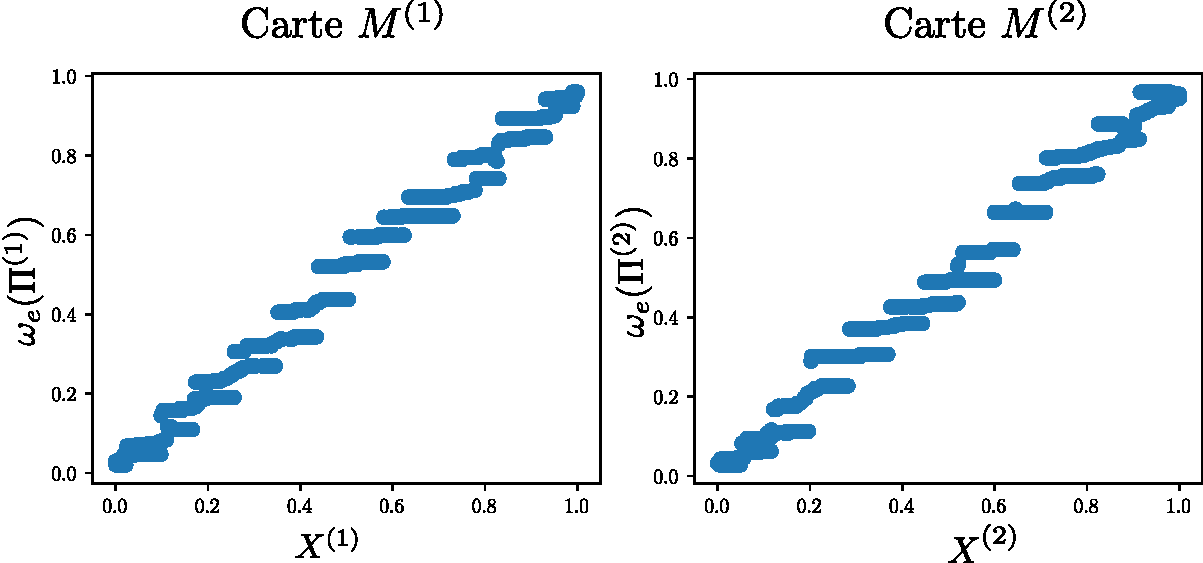
\includegraphics[width=0.7\textwidth]{w_x.pdf}
    \caption{Poids du BMU dans chaque carte en fonction de l'entrée présentée. On s'attend à des tracés proches de l'identité, montrant que le poids du BMU d'une carte est une bonne représentation de l'entrée. Sur ce graphique, on se rapproche effectivement de la fonction identité, cependant, une faible erreur est observée. On observe également un découpage des poids en bandes.\label{fig:erreur}}
\end{figure}


\subsection{Cartographie des entrées}

En biologie, les aires du cortex cérébral sont cartographiées en faisant varier le motif d'entrée dans son espace, et en indiquant, pour chacune des valeurs prises par cette entrée, le neurone y réagissant. Cela donne alors une représentation cartographique où des valeurs de l'espace d'entrée sont tracées par rapport à la positions sur le substrat neuronal du neurone qui y  a réagi.
Par exemple, une carte corticale est tracée pour l'aire visuelle primaire du cortex cérébrale, l'aire v1, en figure~\ref{fig:v1_repr}.

De façon similaire, nous tracerons, pour chaque élément de l'échantillon test, la valeur de l'entrée $\inpx\m{i}$ d'une carte par rapport à la position du BMU $\bmu\m{i}$ qui a été trouvée par le processus de relaxation.
Cette représentation permet d'analyser la quantification des entrées par la carte. En les représentant sur le même graphique, nous mettrons ces éléments en relation avec les poids des cartes en faisant également apparaître les poids externes et contextuels de la carte $M\m{i}$.
%Ces tracés sont réalisables pour des cartes une et deux dimensions et pour des entrées quelconques, que ce soient des réels ou des entrées de plus grande dimension comme des images.
On s'attend à ce que les points soient proches de la courbe des poids externes de la carte $M\m{i}$.
Ce tracé fait également apparaître les zones dans lesquelles les neurones ne sont jamais best matching unit, les \emph{zones mortes}.

Sur le même graphique, nous affichons non seulement les couples $(\bmu\m{i},\inpx\m{i})$ mais également les entrées des autres cartes, également en fonction de $\bmu\m{i}$.
En figure~\ref{fig:inputs}, nous avons ainsi tracé les points $(\bmu\m{1},\inpx\m{1})$ et $(\bmu\m{1},\inpx\m{2})$ issus de l'expérience sur les deux cartes, ainsi que les poids de la carte $M\m{1}$.
Deux valeurs issues de l'échantillon de test sont signifiées en couleur rouge et bleue sur chaque graphique. Un point de même couleur correspond à la même itération de test dans chaque graphique. Ces deux points partagent la même abscisse, donc l'entrée $X\m{1}$ est la même pour ces deux échantillons. Par contre, leur ordonnée est différente et $M\m{2}$ reçoit donc une entrée $\inpx\m{2}$ différente dans ces deux itérations.

Ce tracé nous permet d'abord d'observer que les points $(\bmu\m{1},\inpx\m{1})$ sont proches de la courbe de poids externe: le poids d'un BMU est proche de l'entrée qui a été présentée, le poids du BMU est donc une bonne approximation de cette entrée. Cela permet de conclure que la quantification vectorielle est bien réalisée dans cette carte sur les entrées externes.

Tracer les échantillons de test permet ensuite d'observer la répartition des BMUs sur la carte. Les courbes de poids externes de la carte dans CxSOM (c) et de la carte indépendantes (b) sont indifférenciables; par contre, l'affichage de l'échantillon de test fait apparaître des zones mortes. Nous observons ainsi que la carte au sein de CxSOM est découpée en plusieurs zones dans lesquelle les unités sont BMUs, séparées par des petites zones mortes. Ce tracé permet donc d'identifier un comportement nouveau à investiguer.


En s'intéressant aux valeurs des entrées, nous observons aussi que les BMUs d'une même zone encodent des entrées sur un intervalle réduit, mais que les intervalles encodés par deux zones adjacentes se recoupent. Les points rouges et bleus, ayant la même valeur de $\inpx\m{1}$, sont par exemple envoyés dans deux zones différentes.

Ces valeurs peuvent être mises en relation avec celles de l'entrée $\inpx\m{2}$, également disposées selon $\bmu\m{1}$. Nous pouvons alors observer que deux zones adjacentes de la carte encodent des entrées proches selon $\inpx\m{1}$, mais très différentes pour $\inpx\m{2}$. Cela explique la séparation du point rouge et du point bleu dans deux zones.

La représentation des valeurs d'entrées $\inpx\m{i}$ selon la position du BMU calculée $\bmu\m{i}$ permet ainsi d'identifier une répartition des BMUs sur la carte que nous ne pourrions pas observer en traçant simplement les poids.

\begin{figure}
    \centering
    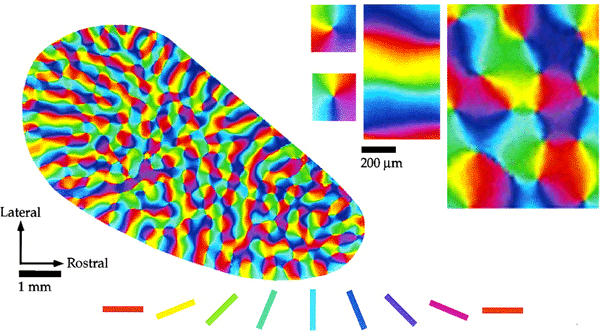
\includegraphics[width=0.7\textwidth]{v1.jpg}
    \caption{Carte corticale de l'aire cérébrale visuelle V1. Pour tracer cette représentation, un ensemble de traits de différentes orientation sont présentés en stimuli visuels au sujet, indiqués en bas de l'image. Le neurone réagissant à une entrée d'orientation particulière est coloré sur la carte de la couleur correspondante à l'entrée. Cette méthode permet de tracer des \emph{cartes corticales} d'une aire cérébrale \cite{Bosking1997OrientationSA}. \label{fig:v1_repr}}
\end{figure}

\begin{figure}
\begin{minipage}{0.27\textwidth}
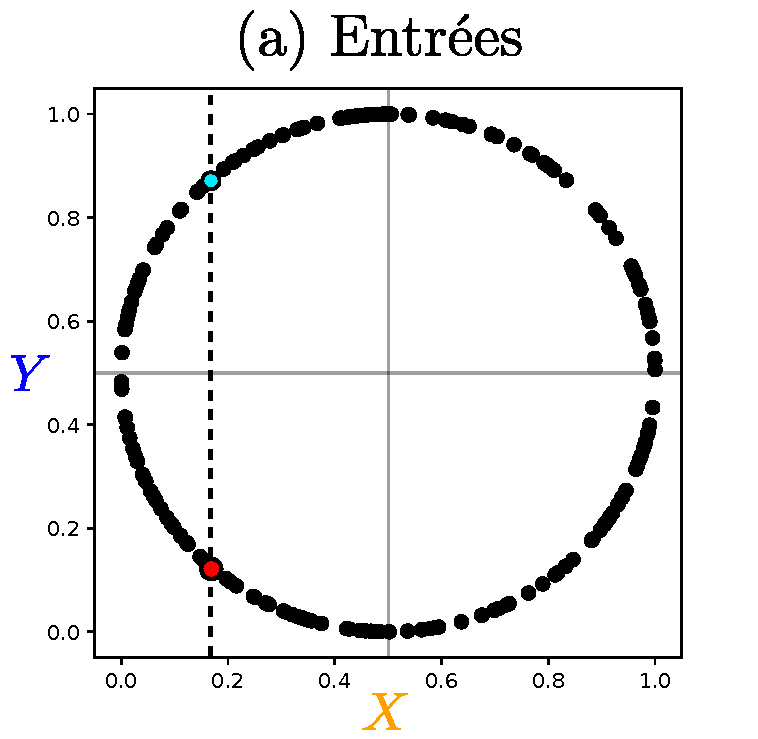
\includegraphics[width=\textwidth]{2som_inp_noU.pdf}
\end{minipage}
\begin{minipage}{0.34\textwidth}
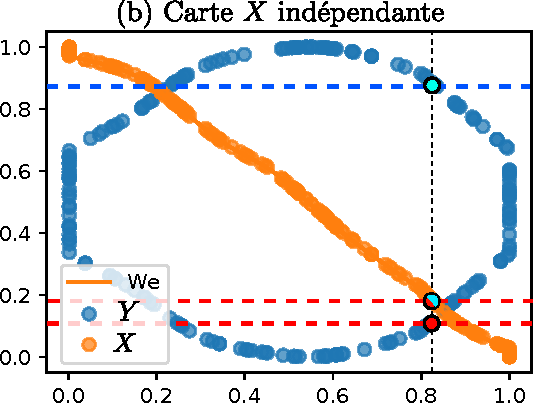
\includegraphics[width=\textwidth]{weights_2som_unco.pdf}
\end{minipage}
\begin{minipage}{0.38\textwidth}
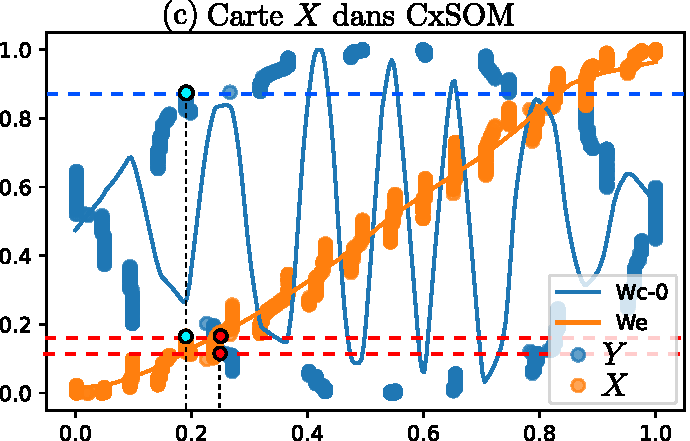
\includegraphics[width=\textwidth]{weights_2som.pdf}
\end{minipage}

\caption{Représentation des entrées $X$,$Y$ d'une architecture de deux cartes relativement au BMU de la carte $X$ après apprentissage. Ces tracés mettent en valeur l'organisation des cartes, différentes dans le cas ou les cartes apprennent indépendemment leurs entrées~(b) ou sont connectées~(c). Les entrées correspondantes sont en figure~(a). Les points bleu et rouge reportés sur les tracés correspondent au même échantillon de test.\label{fig:inputs}}
\end{figure}

\subsection{Représentation du modèle par la variable cachée $U$}

Nous avons vu lors de la représentation cartographique des entrées que chacune des cartes s'organise en fonction non seulement de son entrée externe, mais aussi de l'entrée de l'autre carte. Chaque carte s'organise donc en fonction du \emph{modèle d'entrée}, donc en fonction de $U$.
Nous tracerons les nuages de points $U$ en fonction de la position $\bmu\m{i}$ du BMU d'une carte pour représenter comment la position du BMU traduit la relation entre les entrées. Dans le cas de l'expérience à deux cartes, $U$ est en une dimension.

En figure~\ref{fig:piu}, nous tracons donc $U$ en fonction de $\bmu\m{1}$ et $U$ en fonction de $\bmu\m{2}$.
Ce tracé montre $U$ comme une fonction de la position du BMU dans chaque carte, contrairement au cas ou les cartes ne sont pas connectées. Cela traduit bien le fait que chaque carte a appris une représentation du modèle d'entrée et non seulement de son entrée externe.
Dans le cas où les cartes ne sont pas connectées, il y a plusieurs valeurs de $U$ pour un même $\bmu$, une valeur $x$ de $\inpx\m{1}$ correspondant à deux positions sur le cercle.
L'organisation de la carte dans CxSOM rend chaque position $\bmu$ codant pour une seule valeur de $U$, c'est à dire une seule position d'échantillon sur le cercle. $U$ est alors une fonction de $\bmu$, ce qui est représenté en pointillé sur la figure~\ref{fig:piu}. Donc, chaque carte $M\m{1}$ et $M\m{2}$ encode tout le modèle d'entrée, et non seulement l'entrée externe.
La représentation de $U$ selon la position du BMU d'une carte $\bmu\m{i}$ permet de représenter comment la carte $i$ a appris l'ensemble d'entrées $(\inpx\m{1},\inpx\m{2})$ et non seulement son entrée externe. Déterminer si l'architecture a appris le modèle d'entrées revient à vérifier si $U$ est une fonction de $\bmu$ dans chacune des cartes de l'architecture.
 
\begin{figure}
\centering
\includegraphics[width = 0.7\textwidth]{xu_yu_both.pdf}
\caption{Valeur de $U$ en fonction des valeurs du BMU $\bmu\m{i}$ dans chacune des cartes, pour des entrées prises sur le cercle. Sur la première ligne, nous tracons la réponse de chaque carte à son entrée dans le cas ou les cartes ne sont pas connectée. Sur la deuxième ligne, nous traçons la réponse de chaque carte lorsqu'elles ont appris de façon jointe au sein de CxSOM.
$U$ apparaît alors comme une fonction de la position du BMU $\bmu\m{i}$ dans chaque carte, contrairement au cas ou les cartes apprendraient indépendamment sur les mêmes entrées. Cette relation fonctionnelle est symbolisée par les pointillés sur les tracés du bas.}
\label{fig:piu}
\end{figure}


\subsection{Distortion des poids d'une dans l'espace d'entrée complet}

Une représentation utilisée pour les cartes de Kohonen classique est de tracer les poids du graphe qu'est la carte dans l'espace de ses entrées, tel que la figure de droite en~\ref{fig:representation}. Dans CxSOM, chaque carte prend en entrée une seule des modalités. Par contre, il est possible de représenter comment la carte se déplie dans l'espace de toutes les modalités.

Nous définissons alors une façon de représenter le dépliement d'une seule carte de CxSOM dans l'espace global des entrées. Pour les entrées 2D, il s'agit alors de représenter le dépliement de $M\m{1}$ dans l'espace des entrées $\inpx\m{1},\inpx\m{2}$.

\begin{figure}
    \begin{minipage}{0.45\textwidth}
    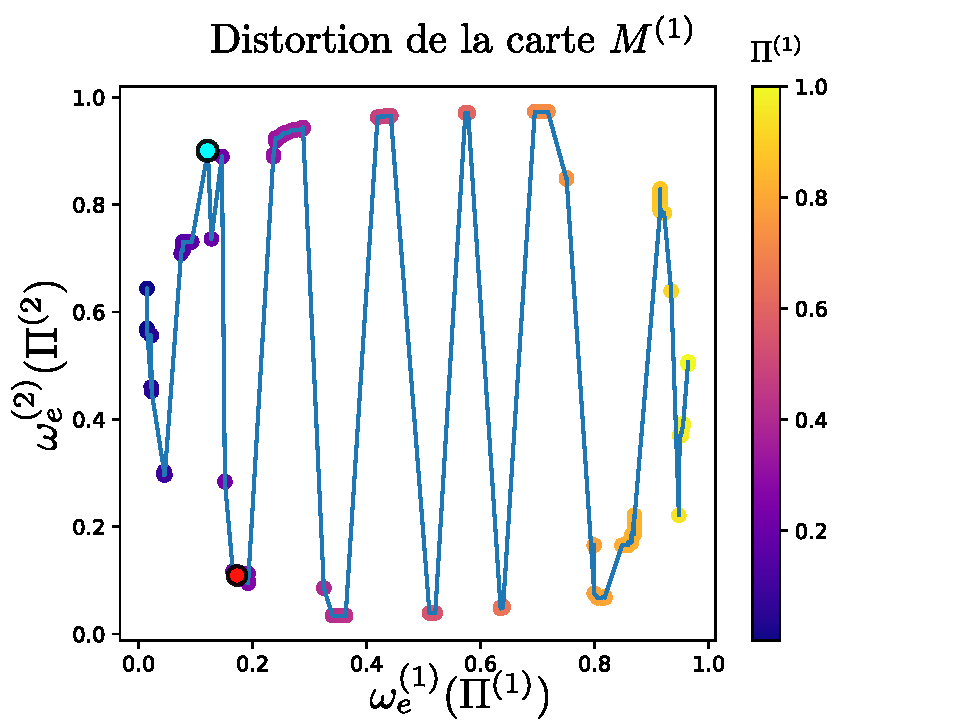
\includegraphics[width=\textwidth]{disto_cercle_M1.pdf}
    \end{minipage}
    \begin{minipage}{0.45\textwidth}
    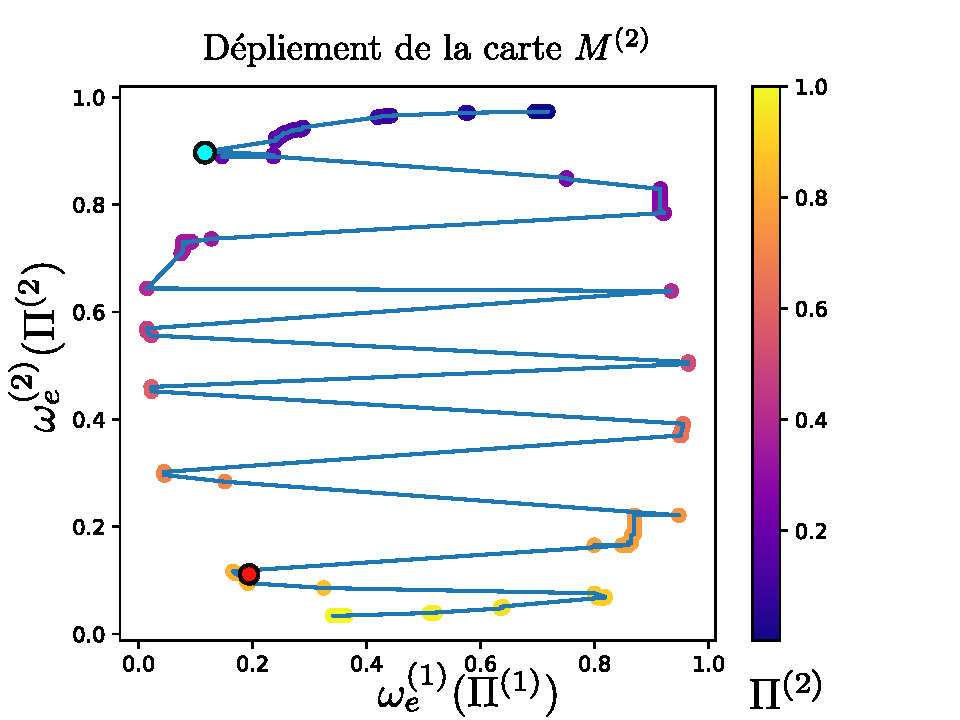
\includegraphics[width=\textwidth]{disto_cercle_M2.pdf}
    \end{minipage}
    \caption{représentation des poids des BMUs des cartes $M\m{1}$ et $M\m{2}$, reliés dans l'ordre de leurs positions selon $M\m{1}$ figure de gauche et $M\m{2}$ figure de droite. Le dépliement de chacune des cartes est alors représenté dans l'espace complet des entrées \label{fig:distortion}}
    \end{figure}

\subsection{Conclusion}

Nous utiliserons donc quatre représentations des cartes dans la suite de cette thèse, toutes définies à partir d'un échantillon de test.
Le tracé du poids du BMU en fonction de l'entrée externe permet d'évaluer comment une carte a individuellement appris une représentation de son espace d'entrée. 


Pour observer comment l'architecture a appris le modèle d'entrée, nous traçons une représentation cartographique des entrées. Sur un même graphique nous tracons les nuages de points $(\inpx\m{1},\bmu\m{1})$ et $(\inpx\m{2},\bmu\m{1})$, de même pour $M\m{2}$, superposés avec les courbes de poids de $M\m{1}$ (respectivement $M\m{2}$). Cette représentation permet d'observer quelles valeurs d'entrées chaque position de BMU encode.

Enfin, nous réduisons si possible la dimension du modèle d'entrée $(\inpx\m{1},\cdots,\inpx\m{n})$ en une valeur $U$ et traçons les nuage de points $(U,\bmu\m{1})$ et $(U,\bmu\m{2})$. L'apprentissage du modèle d'entrée doit se traduire par l'observation d'une relation fonctionnelle entre $U$ et $\bmu$ dans chaque carte.



\section{Un indicateur de l'apprentissage du modèle par l'architecture basé sur l'information mutuelle}

Nous avons présentés différents tracés permettant de conclure que l'architecture de carte a appris une représentation du modèle d'entrée. Cet apprentissage du modèle se caractérise notamment par le fait que chaque carte dissocie ses BMUs en fonction du modèle d'entrée globale et non seulement de son entrée externe. 
Nous souhaitons définir un indicateur numérique caractérisant cet apprentissage. Cet indicateur nous permettra de comparer de multiples expériences entre elles. Les tracés sont réalisables pour une variable cachée $U$ en en une dimension; un indicateur numérique nous permettra aussi d'évaluer l'apprentissage lorsque la dimension de $U$ est plus grande.

Nous avons défini les expériences en termes de variables aléatoires. La théorie de l'information de Shannon \cite{Shannon1948AMT} apporte un modèle mathématique qui permet de manipuler et encoder ces variables et quantifier l'information partagée entre leurs distributions.
Nous définirons dans cette partie un indicateur permettant d'évaluer l'apprentissage du modèle par l'architecture de cartes par des outils d'information. Nous présenterons également la méthode d'estimation choisie. 

\subsection{Information mutuelle et entropie}

Les notions d'\emph{entropie} et les valeurs associées, telle que l'\emph{information mutuelle} entre des distributions, sont des notions fondamentales de la théorie de l'information de Shannon. Ces quantités donnent des informations concernant la distribution d'une variable aléatoire.
Les formules indiquées dans ce paragraphe concernent des variables aléatoire discrètes mais sont transposables en version continue.
L'entropie de Shannon d'une variable aléatoire $X$ à valeurs discrètes dans un ensemble $E_X$, de distribution $p$, est notée $H(X)$ et définie par la formule : 
\begin{equation}
H(X) = - \sum_{x \in E_X}{p(x)\textrm{log}(p(x))}
\end{equation}

Elle se mesure en $bit/symbole$ lorsque le logarithme est en base 2, ce qui est généralement utilisé. 
L'entropie est une mesure de la quantité d'incertitude, ou de surprise, sur la valeur de la variable aléatoire $X$. Si la la distribution de probabilité de $X$ est concentrée autour d'un point, l'entropie est faible : lors d'une réalisation de $X$, l'observateur est \emph{plutôt certain} du résultat. En revanche, l'entropie est maximale lorsque lorsque $X$ suit une distribution de probabilité uniforme.
L'entropie s'interpète également comme la quantité moyenne d'information à fournir, en bits, pour coder la valeur que prend la variable $X$.
De la même manière, on peut définir l'entropie conjointe de deux variables, qui est l'entropie de leur distribution jointe, et l'entropie conditionnelle, qui est l'entropie de leurs distributions conditionnelles.

Outre les entropies jointes et conditionnelles, les relations statistques entre deux variables aléatoires $X,Y \in E_X,E_Y$ peuvent être mesurées par \emph{l'information mutuelle}. Elle se définit formellement par : 
\begin{equation}
 I(X,Y) = \sum_{x,y \in E_X,E_Y}{p(x,y)\textrm{log}(\frac{p(x,y)}{p(x)p(y)})}
\end{equation}
Cette valeur mesure la quantité d'information moyenne apportée par une réalisation de $X$ sur la réalisation de $Y$.

L'information mutuelle possède les propriété suivantes:
\begin{enumerate}
\item $I(X,Y) = 0 \Leftrightarrow \textrm{X et Y sont indépendantes}$. L'information mutuelle peut être vue une mesure de la distance entre la distribution jointe de $(X,Y)$, $p(X,Y)$ et la distribution dans laquelle les deux variables sont indépendantes, $p(X)p(Y)$.
\item Elle s'exprime à partir de l'entropie : $I(X,Y) = H(X) + H(Y) - H(X,Y) = H(X) - H(X|Y) = H(Y) - H(Y|X)$
\item Elle est symétrique : $I(X,Y) = I(Y,X)$
\item Pour toute fonction $f$, $I(X,Y) \geq I(X,f(Y))$. L'égalité est atteinte si et seulement si $f$ est \emph{bijective}.
\end{enumerate}

Lors de l'analyse de CxSOM, on s'interroge sur l'information que portent les positions des BMUs $\bmu$ d'une carte sur le modèle d'entrée. Les éléments de la carte ont été définis en termes statistiques; on peut donc utiliser l'information mutuelle comme une représentation de l'information portée par le BMU d'une carte sur le modèle d'entrée.
\subsection{Indicateur}

Nous avons introduit $U$, la variable correspondant à une réduction de dimension des entrées $(\inpx\m{i})$. Dans l'exemple, $U$ est en une dimension pour des entrées 2D $(\inpx\m{1},\inpx\m{2})$.
Nous avons observé que si l'architecture a appris le modèle s'entrée, alors $U$ est une fonction de $\bmu$ dans chacune des cartes.
Cette relation fonctionnelle montre qu'une carte a appris non seulement une représentation de son entrée mais aussi une représentation du modèle complet, représenté par $(\inpx\m{1},\cdots,\inpx\m{n})$ ou par la variable $U$, qui est en bijection avec $(\inpx\m{1},\cdots,\inpx\m{n})$.
Nous cherchons à définir un indicateur permettant d'évaluer l'apprentissage du modèle par l'architecture de cartes. D'après les observations mentionnées ci-dessus, nous cherchons donc un indicateur traduisant le fait que $U$ est une fonction de $\bmu$ dans chacune des cartes. Nous attendons que cet indicateur prenne une valeur minimale lorsque $U$ n'a aucune relation avec $\bmu$, et augmente jusqu'à une valeur maximale lorsque $U$ est fonction de $\bmu$. Afin de pouvoir comparer les expériences entre elles, nous voulons définir un indicateur normalisé, dont la valeur est donc comprise entre $0$ et $1$.


Nous pouvons utiliser $I(\bmu, U)$ comme l'information moyenne qu'une position de BMU d'une carte porte sur $U$, donc sur le modèle d'entrées, et $U$ sur le BMU.  Il est alors nécessaire ici que la relation entre $U$ et $\mathbf{X}$ soit bijective.
L'information mutuelle dépend de la quantité d'information portée par chaque distribution et se mesure en bit/symbole. Nous cherchons un indicateur normalisé.


Nous choisissons de normaliser l'information mutuelle $I(\bmu,U)$  par la valeur maximale qu'elle peut prendre dans une expérience de CxSOM. Cette valeur maximale atteinte par $I(\bmu,U)$ est $H(U)$, atteinte lorsque $U$ est fonction de $\bmu$.
En effet, par construction, $\bmu$ est une fonction de $U$ dans une carte de Kohonen: l'algorithme est déterministe et une sortie est définie pour toute valeur de $U$. C'est à dire, $I(U,\bmu) = I (U, f(U))$.
Par propriété de l'information mutuelle, pour toute fonction $f$ et variables $X,Y$, $I(X,f(Y)) \leq I(X,Y) $. 
Donc, $I(U,\bmu) \leq I(U,U) = H(U)$
Cette valeur est atteinte si et seulement si $U$ et $\bmu$ sont en bijection, autrement dit, si et seulement si $U$ est aussi une fonction de $\bmu$.

Nous définissons donc un indicateur de la relation fonctionnelle existant entre $U$ et $\bmu$ comme:
\begin{equation}
I_x(U|\bmu) = \frac{I(\bmu,U)}{H(U)}
\end{equation}
Ce coefficient n'est pas symétrique, et mesure donc l'information portée par le premier terme sur le second, relativement à la valeur maximale qu'elle peut prendre. Dans le cas des cartes CxSOM, $I_x \in [0,1]$. Cette valeur rappelle le \emph{coefficient d'incertitude} entre $U$ et $\Pi$ \cite{Theil1961EconomicFA}.


%TODO : développer ce point : information portée par plus de variables !
%TODO : calculer et comparer les valeurs pour le cas du cercle.

Ce coefficient peut être élargi à plus de variables: on peut calculer $I_x(U | (\bmu\m{1},\bmu\m{2},\bmu\m{3}))$ pour 3 cartes, en considérant la variable jointe $(\bmu\m{1},\bmu\m{2},\bmu\m{3})$.
Plus largement, pour prouver que l'archictecture a appris un modèle, on souhaite que $I_x(U|\bmu\m{1},\cdots,\bmu\m{k})$ soit le plus proche possible de 1.

Cet indicateur permet de comparer des expériences par des valeurs numériques, sans passer par des tracés.

\subsection{Estimation}

L'information mutuelle et l'entropie sont des grandeurs probabilistes. Elles sont définies à partir de la distribution des variables aléatoires. Ces distributions, dans notre cas, ne sont pas connues, nous devons donc estimer ces quantités.
Nous passons par une estimation de la distribution des variables $U$,$\bmu$ et la distribution de la variable jointe $(U,\bmu)$ en discrétisant l'espace par la méthode des \emph{histogrammes}.
Cette méthode est représentée en figure~\ref{fig:binning}. Les variables $U$ et $\bmu$ sont discrétisées en \emph{boîtes} de centres $x_k$ et $y_k$.
La distribution de X est alors estimée par: 
$$P(U = x_i) = \frac{n_{xi}}{N} $$ où $n_{xi}$ est le nombre d'échantillons de X tombant dans la boîte de valeur $x_i$ et $N$ le nombre de points. Le même procédé est réalisé pour $\bmu$ et $(U,\bmu)$. La précision de l'estimation peut être améliorée en choisissant des tailles de boîtes variables; nous utilisons ici la méthode simple avec des boites de taille fixe. Pour des variables à valeur dans $[0,1]$, les centres sont définis par $x_k = \frac{k}{M}+\frac{1}{2M}$, avec $M$ le nombre de boîtes.
L'information mutuelle et l'entropie sont ensuite estimées à partir de ces distributions discrètes, par leur formules:
\begin{equation}
    I(U,\bmu) = \sum_{i = 0}^{n_x} \sum_{j=0}^{n_y} {P(x_i,y_j)\textrm{log}\left(\frac{P(U = x_i,\bmu = y_j)}{P(U = x_i)\times P(\bmu = y_j)}\right)}
   \end{equation}

La méthode par histogramme est simple, mais biaisée quand la dimension des entrée augmente.
Le nombre d'échantillons disponibles pour l'estimation doit augmenter exponentiellement avec la dimension des variables pour éviter le phénomène de "boîtes vides": à cause de la dispersion des données, de nombreuses boîte $(x_j,y_i)$ ne contiendront pas de points alors qu'elles auraient dû en contenir selon leur distribution; l'estimation de la distribution en ce point sera alors nulle, et l'estimation de l'indicateur faussée.
\begin{figure}
\centering
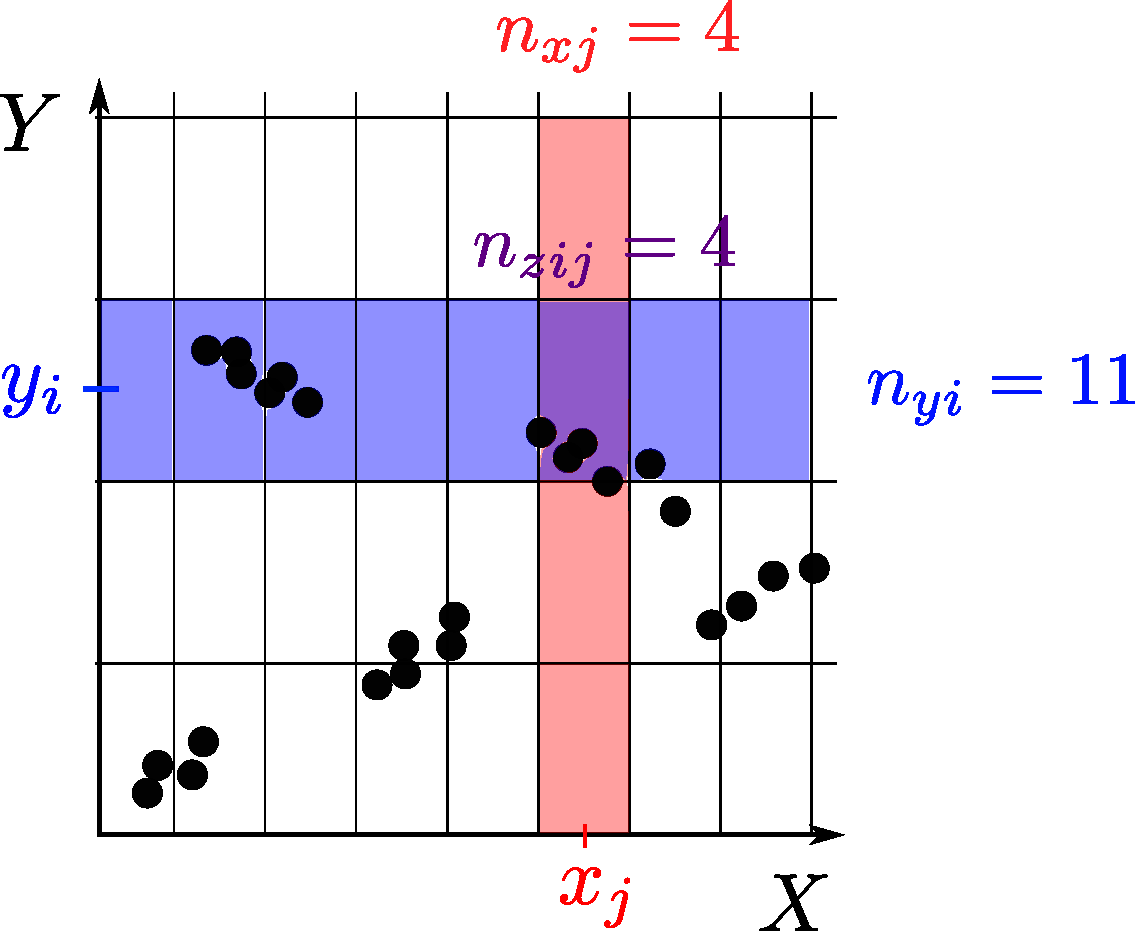
\includegraphics[width=0.45\textwidth]{boxes}
\caption{Méthode par histogrammes pour estimer les distributions des variables $U$ et $\bmu$. Les distributions sont estimées à partir de $n_{xj}$, $n_{yi}$ et $n_{zij}$, puis les valeurs de l'entropie $H$ et l'information mutuelle $I$ calculées.}
\label{fig:binning}



Nous avons donc envisagé d'autres estimateurs moins biaisés en grand dimension. Détaillons par exemple l'estimateur par KNN (K-nearest neighbors) de Kraskov \cite{2004kraskov}. 
Cet estimateur ne passe pas par l'estimation de la densité de probabilité, contrairement aux histogrammes, mais estime directement l'information mutuelle. C'est l'estimation de la densité de probabilité qui posai justement problème en grande dimension.
Le découpage de l'espace se fait en recherchant, pour un couple $(X,Y)$ les k plus proches voisins. Une information mutuelle locale est calculée dans cette zone de l'espace, suivant une formule permettant d'approximer les différences de logarithme par la fonction digamma $\psi$ : 
$$i_j(X,Y) = \psi(k) - \psi(n_{x_j} + 1) - \psi(n_{y_j} +1) + \psi(N)$$
Cette information mutuelle locale est ensuite moyennée sur l'ensemble des points: 
$$\hat{I}(X,Y) = \psi(k) - \langle\psi(n_{x_j} + 1) + \psi(n_{y_j} +1)\rangle + \psi(N)$$
Pour estimer $I_x(X|Y)$, on estimera $I(X,Y)$ et $H(Y)$ avec les mêmes paramètres, en notant que $H(Y) = I(Y,Y)$.
L'estimateur de Kraskov est plus granulaire que la méthode des histogrammes. 

\end{figure}

%\begin{figure}
%\centering
%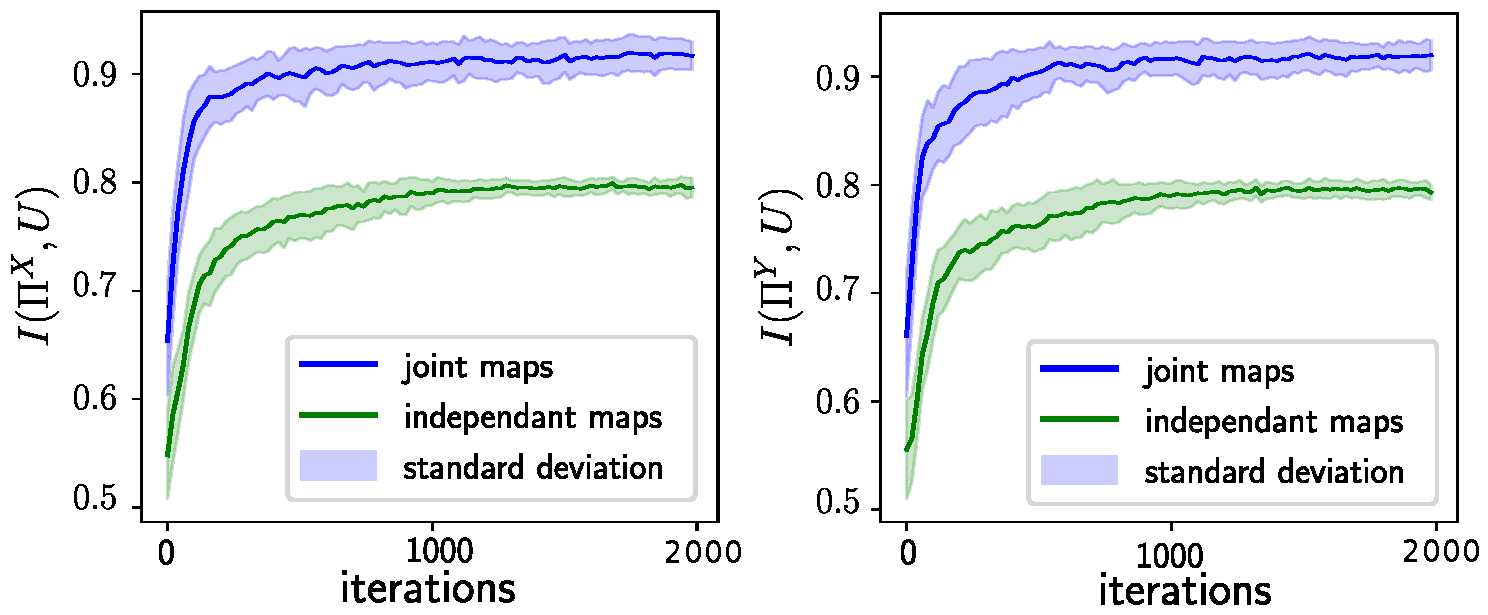
\includegraphics[width=\textwidth]{mutual_info_evol.pdf}
%\caption{Evolution de l'indicateur relatif à l'information mutuelle entre $\Pi$ et $U$ dans chaque carte au cours de l'apprentissage. Cet indicateur est comparé à celui calculé dans le cas ou les cartes apprennent séparément.}
%\label{fig:im} 
%\end{figure}

\subsection{Information mutuelle sur deux cartes}

Le fait d'utiliser un indicateur numérique permet de tracer l'évolution de cet indicateur au cours de l'apprentissage des cartes. Nous traçon cette évolution au cours de l'apprentissage dans un système de deux cartes apprenant sur le cercle en deux dimensions.

Pour cette expérience, une phase de test sur 5000 entrées est réalisée toutes les 10 itérations, puis toutes les 200 itérations à partir de l'itération 200. Chaque phase de test donne alors un ensemble d'entrées $\inpx\m{1}, \inpx\m{2}, U$ et un ensemble de réponses des cartes $\bmu\m{1}, \bmu\m{2}$. On peur alors estimer $I_x(U|\bmu\m{1})$ et $I_x(U|\bmu\m{2})$ sur chaque itération considérée, ce qui nous donne la courbe de l'évolution de l'indicateur au long de l'apprentissage. 
Ces calculs sont réalisés sur 100 apprentissages complets, prenant des entrées d'apprentissage aléatoires sur le même cercle. Les cartes sont initialisées à des poids aléatoires au début de chaque apprentissage. 
Les tracés présentés en figure~\ref{fig:MI_evol}, sont la moyenne, à chaque pas de temps, de l'information mutuelle de chaque expérience au pas de temps $t$. Nous avons représenté ici l'évolution de l'information mutuelle moyenne sur 50 expériences.

L'estimation est réalisée par la méthode des histogrammes. On choisit de découper les valeurs de $U$ en 50 boîtes, et en 500 pour $\bmu\m{i}$; de cette façon, les points correspondant à des $U$ très proches seront comptés ensemble pour l'estimation de l'information..

Nous comparons les valeurs obtenues pour une carte de CxSOM à celles d'une carte apprenant sur les mêmes entrées $\inpx\m{1}$ ou $\inpx\m{2}$, mais sans connexions entre elles. On s'attend à ce que l'information soit plus élevée pour la carte au sein de CxSOM que la carte seule, ce qui montrerait que la carte porte aussi de l'information sur l'autre entrée. On s'attend à ce que cette valeur atteigne 1, ce qui montrerait qu'une seule carte porte de l'information sur tout le modèle: $U$ est une fonction de $\bmu$ dans chaque carte.

L'observation du tracé montre que les quantités $I_x(U|\bmu\m{1})$ et $I_x(U|\bmu\m{2})$ sont bien toutes deux plus élevées à chaque moment de l'apprentissage que dans le cas ou les cartes sont séparées. Ces quantités augmentent au cours de l'apprentissage, traduisant bien un gain d'information des cartes sur le modèle.

\begin{figure}
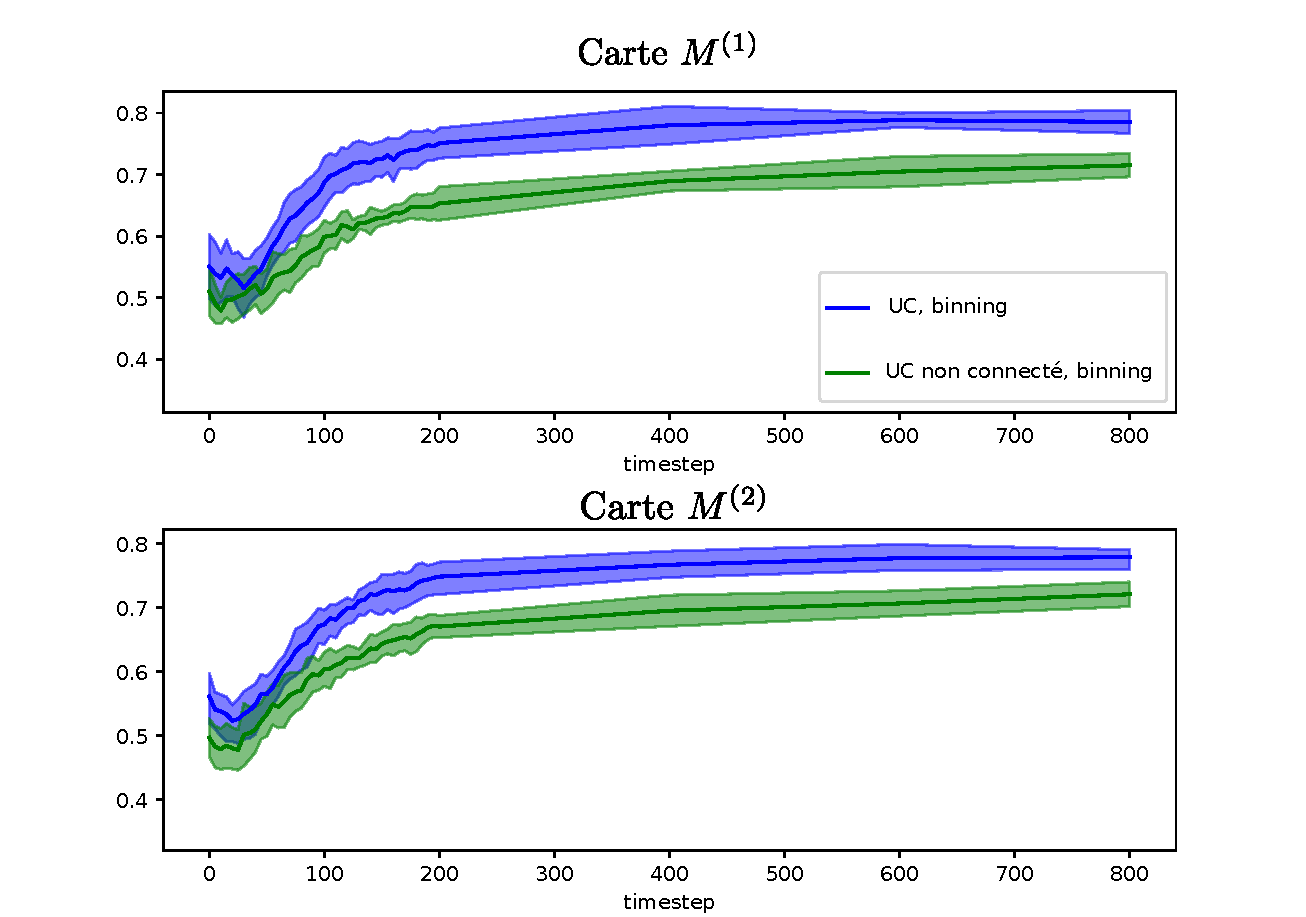
\includegraphics[width=\textwidth]{evolution_MI_binning}
\caption{Evolution du coefficient d'incertitude dans chaque carte au long de l'apprentissage. La courbe bleue correspond à $I_x(U|\bmu)$ dans l'architecture de cartes $M\m{1}$ et $M\m{2}$. On compare cette évolution à l'évolution de l'information d'une seule carte apprenant sur les mêmes entrées $X$ ou $Y$, sans être connectée.}
\label{fig:MI_evol}
\end{figure}

\subsection{Discussion}

\subsubsection{Qualité de l'estimation}

Comparons les deux méthodes d'estimation de l'information mutuelle proposées dans ce chapitre: l'estimation par histogrammes, et l'estimation par KNN de Kraskov.
En figure~\ref{fig:MI_evol_total}, nous tracons l'évolution de l'information mutuelle moyenne, cette fois estimée par la méthode de Kraskov. Sur le même schéma, nous tracons également l'évolution de l'information mutuelle obtenue par la méthode des histogrammes. 

Sur les tracés, l'indicateur calculé avec la méthode de Kraskov converge vers une même valeur à la fin de l'apprentissage pour la carte simple que pour la carte au sein d'une architecture CxSOM (tracés rouges et noirs). Ce résultat est étonnant: cela signifie donc que la carte au sein de CxSOM n'a pas plus d'information sur le modèle que la carte isolée, lorsque cette information est estimée avec la méthode de Kraskov. Ce résultat va également à l'encontre de ce qu'on observe sur l'évolution de l'information mutuelle calculée par les histogrammes, dans laquelle une différence franche est observée entre la carte isolée et la carte au sein de l'architecture.

Proposons une explication.
La méthode des noyaux de Kraskov est plus "granulaire" que la méthode des histogrammes au niveau de l'estimation, c'est à dire que les données sont considérées \emph{points par point}. L'avantage est que l'évaluation de la relation fonctionnelle entre $U$ et $\bmu\m{i}$ est plus précise qu'avec les histogrammes: s'il y a deux valeurs de $U$ pour un même $\bmu\m{i}$, l'information diminue. Par contre, la contribution de ces deux valeurs sera la même dans le calcul de l'information mutuelle, qu'elles soient proches ou éloignées: la distance entre donnée n'intervient pas dans le calcul. Cette différence de contribution est illustrée en figure~\ref{fig:exemple-limite}. On calcule l'information mutuelle $I_x$ dans les deux cas de distribution proposées, à l'aide de l'estimateur granulaire de Kraskov. Dans le cas ou la relation est proche d'une relation fonctionnelle, mais est très bruitée, l'information $I_x(Y|X)$ est plus faible que dans le cas ou cette relation n'est pas fonctionnelle, mais sans bruit parasite.

On observe que l'information $I_x(U|\bmu)$ tend vers une même valeur dans CxSOM et dans une carte isolée quand on la calcule avec l'estimateur granulaire. Cela signifie, qu'on a la même quantité d'information sur $U$ avec le BMU, dans la carte isolée que dans CxSOM. Simplement, cette information n'est pas répartie de la même façon. 
Dans une carte isolée, le niveau de quantification vectorielle qu'on effectue sur $X$ est très précis: lorsqu'on présente une entrée $X$ à la carte, le poids du BMU est très proche de cette valeur $X$ Dans CxSOM, on perd ce niveau de quantification, ce qu'on a observé en figure~\ref{fig:erreur}. Le fait que l'indicateur, lorsqu'il est estimé avec une méthode très granulaire, prend la même valeur dans les deux expériences traduit alors qu'on a perdu de l'information sur l'entrée $X$ par rapport à la carte isolée, avec la perte de précision, mais qu'on a gagné de l'information sur l'autre entrée $Y$. Le fait que les deux évolutions de $I_x$, pour chaque expérience, convergent vers la même valeur montre qu'on est dans une situation de compromis: on gagne de l'information sur le modèle au détriment de l'information sur l'entrée externe.

C'est donc le fait de discrétiser grossièrement la distribution de $U$ qui permet de mesurer le gain d'information sur le modèle complet, sans prendre en compte le fait que la précision sur l'entrée externe est affaiblie. L'indicateur $I_x$ reste un indicateur fiable, mais il doit être utilisé en prenant en compte cet aspect.

%ela a peu de sens dans le cas de notre application: on souhaite mesurer que $U$ est proche d'une fonction de $\bmu$, mais du bruit est toléré. L'estimation par histogrammes permet de ne pas prendre en compte ce bruit; ce n'est pas possible avec la méthode de Kraskov. 



\begin{figure}
    \centering
    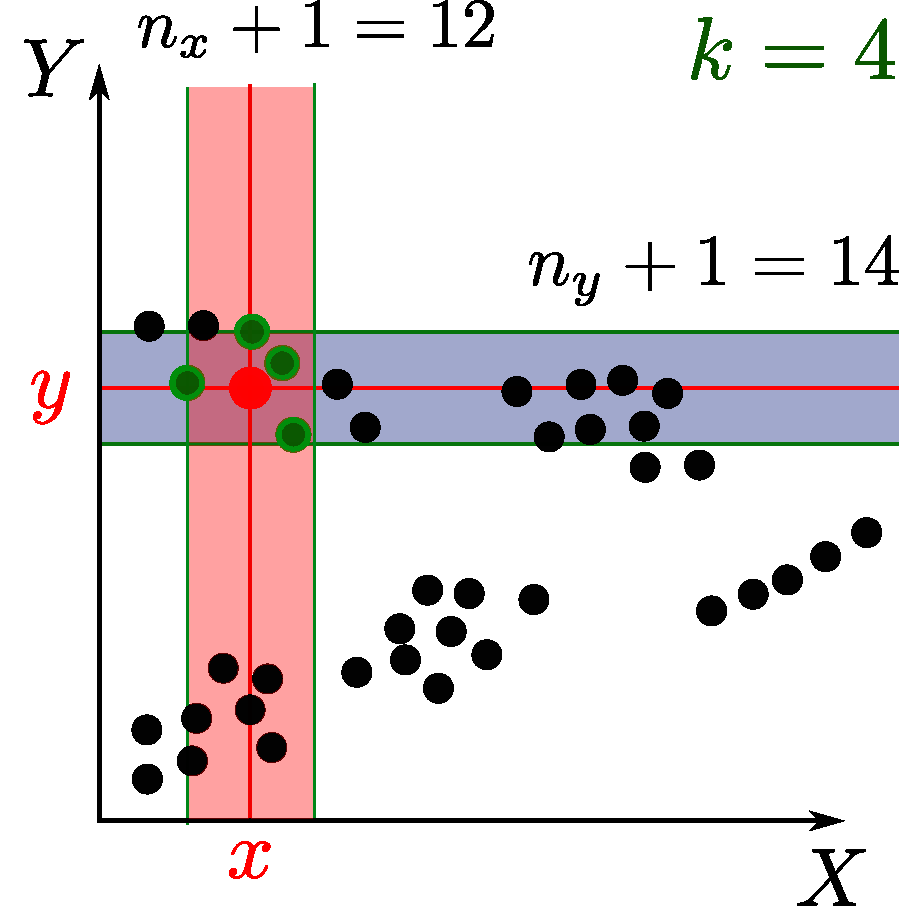
\includegraphics[width=0.35\textwidth]{kraskov.pdf}
    \caption{Découpage en KNN de Kraskov pour estimer l'entropie et l'information mutuelle des variables $X$ et $Y$. Les plus proches voisins du point rouge sont trouvés, en vert, et le processus est répété sur tous les points. Les valeurs de $n_x$ et $n_y$ permettent d'estimer directement l'entropie.}
    \label{fig:kraskov}
\end{figure}

\begin{figure}
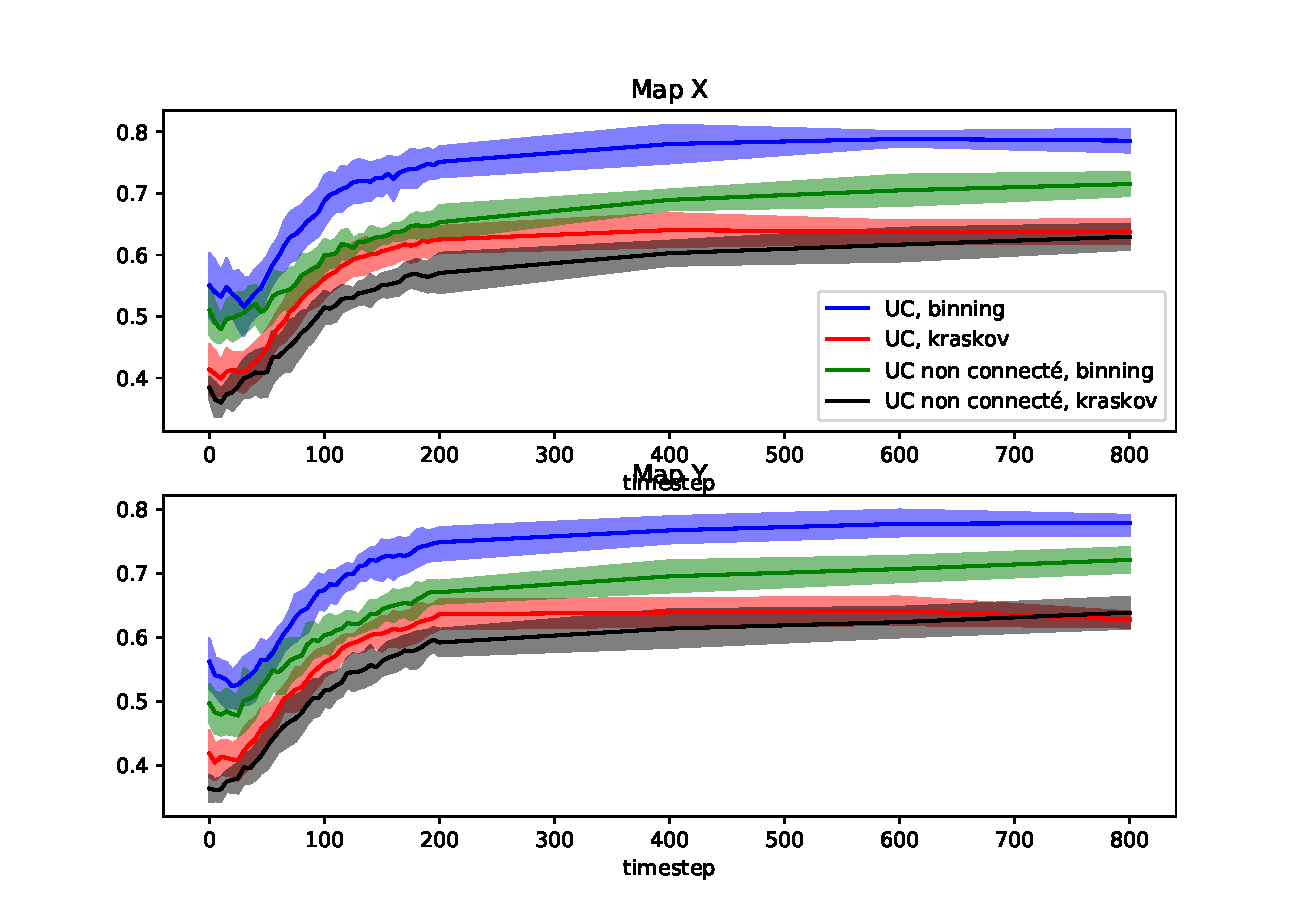
\includegraphics[width=\textwidth]{evolution_MI}
\caption{Evolution du coefficient d'incertitude dans chaque carte au long de l'apprentissage, en comparant l'estimation par histogrammes et l'estimation par la méthode de Kraskov.}
\label{fig:MI_evol_total}
\end{figure}

\begin{figure}
    \centering
    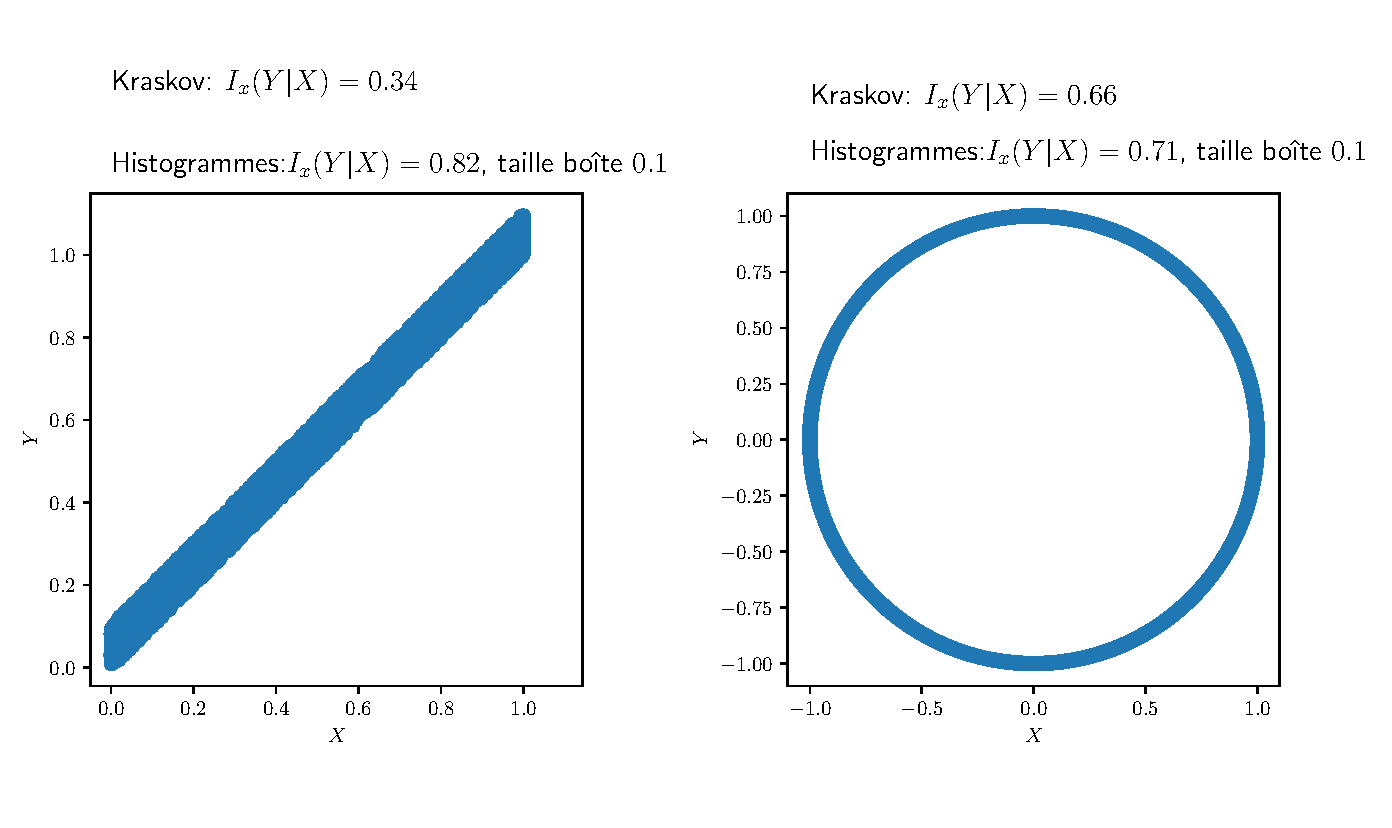
\includegraphics[width=\textwidth]{comparaison_binning_kraskov.pdf}
    \caption{Comparaison du calcul de l'indicateur $I_x$ sur deux distributions. A gauche, la relation entre $Y$ et $X$ se rapproche d'une fonction, mais bruitée. A droite, la relation n'est pas fonctionnelle, mais de telle sorte qu'une valeur de $X$ correspond au maximum à deux valeurs de $Y$. Lorsqu'on calcule l'indicateur avec la méthode très granulaire de Kraskov, cet indicateur est plus élevé dans le cas de droite que de gauche: en effet, le calcul ne prend pas en compte si les points sont condensés ou éloignés. Pour que l'indicateur nous informe correctement sur l'aspect fonctionnel de la relation entre $X$ et $Y$, il faut enlever manuellement le bruit. Avec la méthode par histogrammes, on prend une taille de boîte de $0.1$ selon $Y$. Dans ce cas, l'indicateur est bien plus élevé à gauche, ou $Y$ se rapproche d'une fonction de $X$, que à droite.}
    \label{fig:exemple-limite}
    \end{figure}

\subsubsection{Perspectives}

L'indicateur $I_x$ permet donc bien de mesurer s'il existe une relation fonctionnelle entre $U$ et la positio du BMU d'une carte. Cependant, son estimation doit nécessairement être réalisée par histogrammes, avec une grande taille de découpage pour $U$. Ce découpage occulte le fait qu'une position de BMU code pour une zone de valeur de $U$ plus grande que pour une carte classique. 

L'estimation du même indicateur par une méthode plus granulaire et précise nous informe sur le comportement d'une carte.

L'indicateur que nous proposons, $I_x(Y|X) = \frac{I(X,Y)}{H(Y)}$ traduit bien le fait que les cartes ont appris une relation entre les entrées. Son estimation doit passer par une discrétisation avec des intervalles larges pour $U$, afin de ne pas prendre en compte la perte d'information sur l'entrée externe $X$.
Les données doivent égalemement être débruitées avant l'estimation.
Cet indicateur permet de comparer les expériences entre elles.
L'information mutuelle et l'entropie étant des quantités fondamentales en théorie de l'information, il existe de nombreuses méthodes d'estimations de ces valeurs malgré la difficulté qu'elle pose, voir~\cite{Doquire2012ACO} pour une revue de différentes méthodes. Ainsi, l'utilisation du coefficient d'incertitude comme indicateur reste robuste pour des données de plus grande dimension ou pour plus de cartes, en utilisant des méthode d'estimations plus élaborées. Cependant, cette estimation devra être retravaillée en plus grande dimension. 

\draft{
Une solution serait par exemple de chercher à séparer les sources d'information: l'information apportée par $X$ sur $U$ de l'information apportée par $\bmu$ sur $U$. On pourrait alors mesurer un gain d'information. Par exemple, en~\cite{williams_nonnegative_2010}, les auteurs décomposent l'information à plusieurs variables en \emph{redondance} et \emph{synergie}. 
}


% \draft{
% \subsection{Autre indicateur: le ratio de core}

% L'indicateur correlation ration permet de mesurer la distance d'une distribution à la fonction qui la fitte. Cela correspond bien à ce qu'on cherche dans CxSOM, mais estimation complexe aussi en grand dimension. 
% }

\section{Conclusion}
\begin{itemize}
\item La représentation par échantillonnage et variable aléatoire permet de mieux comprendre les mécanismes des cartes, ceux ci ne reposant plus directement sur les courbes de poids
\item Ces tracés montrent qu'une architecture de deux cartes s'organise comme une carte simple, mais modulée par l'entrée contextuelle: les poids externes se déplient comme une carte simple, mais les poids contextuels amènent des zones dans la carte. Ces zones séparent les BMUs en fonction de à la fois les entrées externes (organisation générale), et des entrées contextuelles (localement). Observation d'un nombre réduit de zones. 
\item Perte de précision au niveau de la quantification des poids externes, mais apprentissage d'un modèle. Nécessité de faire un compromis, réalisé de façon auto-organisée. Chaque carte a alors appris le modèle en entier et non seulement son entrée.
\item Utilisation d'un indicateur basé sur l'info mutuelle pour évaluer comment une carte apprend le modèle. Indicateur pouvant être utile en grande dimension ; mais l'estimation peut poser problème à ce moment.
\end{itemize}


\comment{Correlation ration : mesure de dépendance fonctionnelle
Débruitage de l'IM : répétition de l'expérience et moyenne ?}
\draft{Le ration de corrélation traduit mieux que le coefficient d'incertitude la dépendance fonctionnelle entre le modèle et le BMU. Cependant, à l'inverse de l'information mutuelle, une relation non fonctionnelle mais précise (telle que l'exemple du cercle de la figure~\ref{fig:exemple-limite}) entre les variables aura un score très faible. Ce n'est pas non plus voulu. 

Il semble que l'information mutuelle reste le moyen le plus prometteur et le plus général de mesurer la relation entre les éléments des cartes. Dans le cas une dimension, on observe qu'on veut tendre vers U fonction du BMU; on connait mal le comportement recherché en dimension plus grande (cartes 2D, entrées de grande dimension). L'information mutuelle laisse donc l'opportunité à plus d'états d'organisation des cartes de l'architecture d'avoir un bon score. La meilleure perspective serait donc de pouvoir calculer le coefficient d'incertitude sur des échantillons provenant de données non bruitées, ou de pouvoir séparer le bruit des données lors du calcul du coefficient.
Dans cette optique, l'estimateur par histogrammes permet de réduire l'effet du bruit, en choisissant correctement les tailles de boîtes. L'utilisation histo versus Kraskov reste donc à discuter.
Dans le cas ou le modèle d'entrée est connu, calculer les réponses des cartes sur des jeux de données non bruitées générées artificiellement, après apprentissage sur un jeu de données réelles et bruitée, est une solution. Si le modèle n'est pas connu, des méthodes statistique de réduction de bruit peuvent être imaginées.} 

\draft{
\section{Prédiction d'entrée}

Au sein d'une architecture de cartes, il est possible de ne pas présenter à une ou plusieurs cartes de l'architecture leur entrée externe $\inpx\m{i}$. Dans ce cas, une best matching unit peut quand même être calculée par leurs entrées contextuelles. Le poids de cette best matching unit peut alors être vu comme une prédiction de l'entrée manquante. Cette capacité de prédiction peut être à la fois vue comme une application possible de l'architecture, mais aussi comme une façon de représenter \emph{ce que les autre cartes connaissent d'une autre}. Tracer les prédictions d'une carte est donc un indicateur de la façon dont une architecture a appris des relations. 


\comment{
2 parties dans estimation/perspectives : 
d'une part, questionnement sur l'estimation des données bruitées par exemple - pas besoin de proposer des solutions si elles ne sont pas testées ? 
Et parler de l'estimation en grande dimension : ce n'est pas forcément le pb ici. Donc pas la peine...
}
}
